\chapter{LAN Architectures}\label{lan-architectures}

\begin{itemize}
\tightlist
\item
  You have studied various NETWORK technologies: ROUTING, SWITCHING,
  STP, ETHERCHANNEL, OSPF, FHRPs, SWITCH SECURITY FEATURES, etc.

  \begin{itemize}
  \tightlist
  \item
    Now, let's look at some BASIC NETWORK DESIGN / ARCHITECTURE
  \end{itemize}
\item
  There are standard ``BEST PRACTICES'' for NETWORK DESIGN

  \begin{itemize}
  \tightlist
  \item
    However there are a few UNIVERSAL ``CORRECT ANSWERS''
  \item
    The answer to MOST general questions about NETWORK DESIGN is ``IT
    DEPENDS''
  \end{itemize}
\item
  In the early stages of your NETWORKING career, you probably won't be
  asked to DESIGN NETWORKS yourself
\item
  However, to understand the NETWORKS you will be CONFIGURING and
  TROUBLESHOOTING, it's important to know some BASICS of NETWORK DESIGN
\end{itemize}

\section{Common Terminologies}\label{common-terminologies}

\begin{itemize}
\tightlist
\item
  STAR

  \begin{itemize}
  \tightlist
  \item
    When several DEVICES all connect to ONE CENTRAL DEVICE, we can draw
    them in a ``STAR'' shape like below, so this is often called a
    ``STAR TOPOLOGY''
  \end{itemize}
\end{itemize}

\begin{figure}
\centering
\pandocbounded{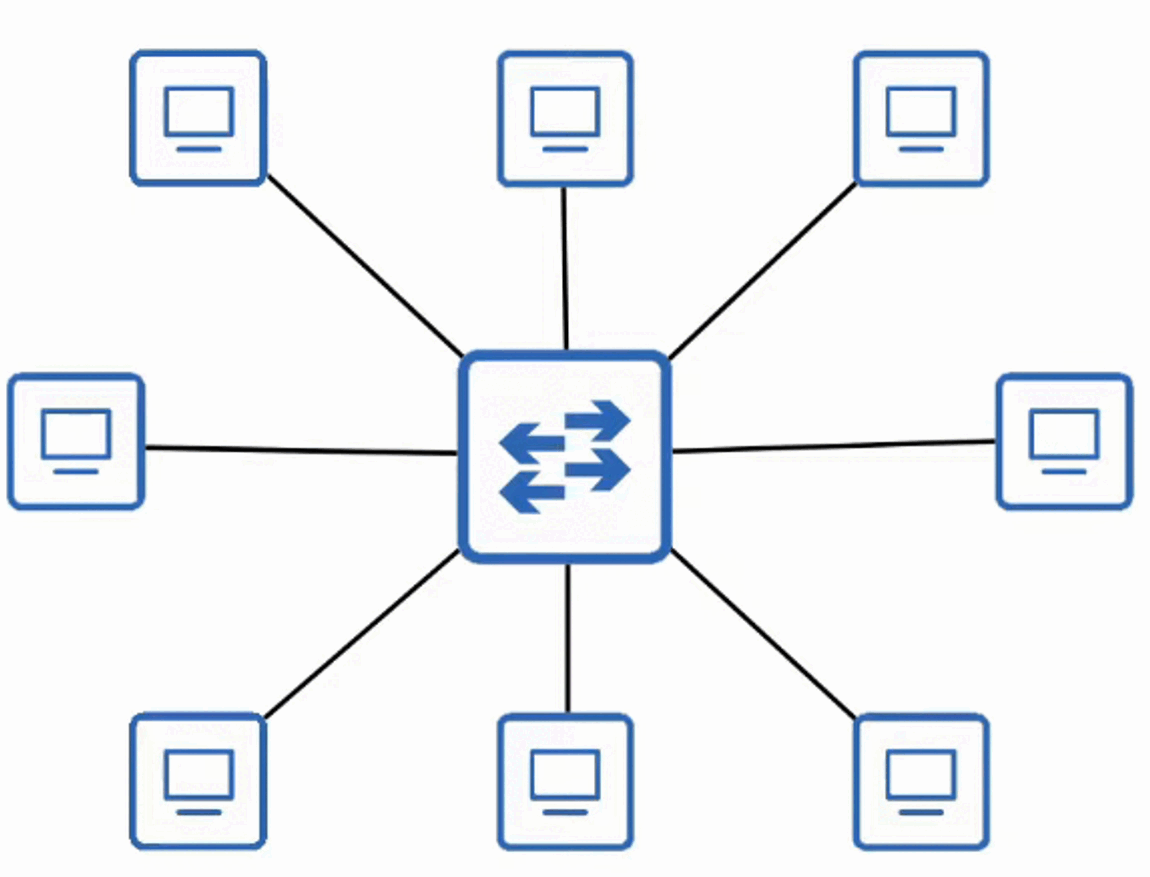
\includegraphics[keepaspectratio,alt={image}]{images/53-lan-architectures/img-001.png}}
\end{figure}

\begin{itemize}
\tightlist
\item
  FULL MESH

  \begin{itemize}
  \tightlist
  \item
    When each DEVICE is connected to each OTHER DEVICE
  \end{itemize}
\end{itemize}

\begin{figure}
\centering
\pandocbounded{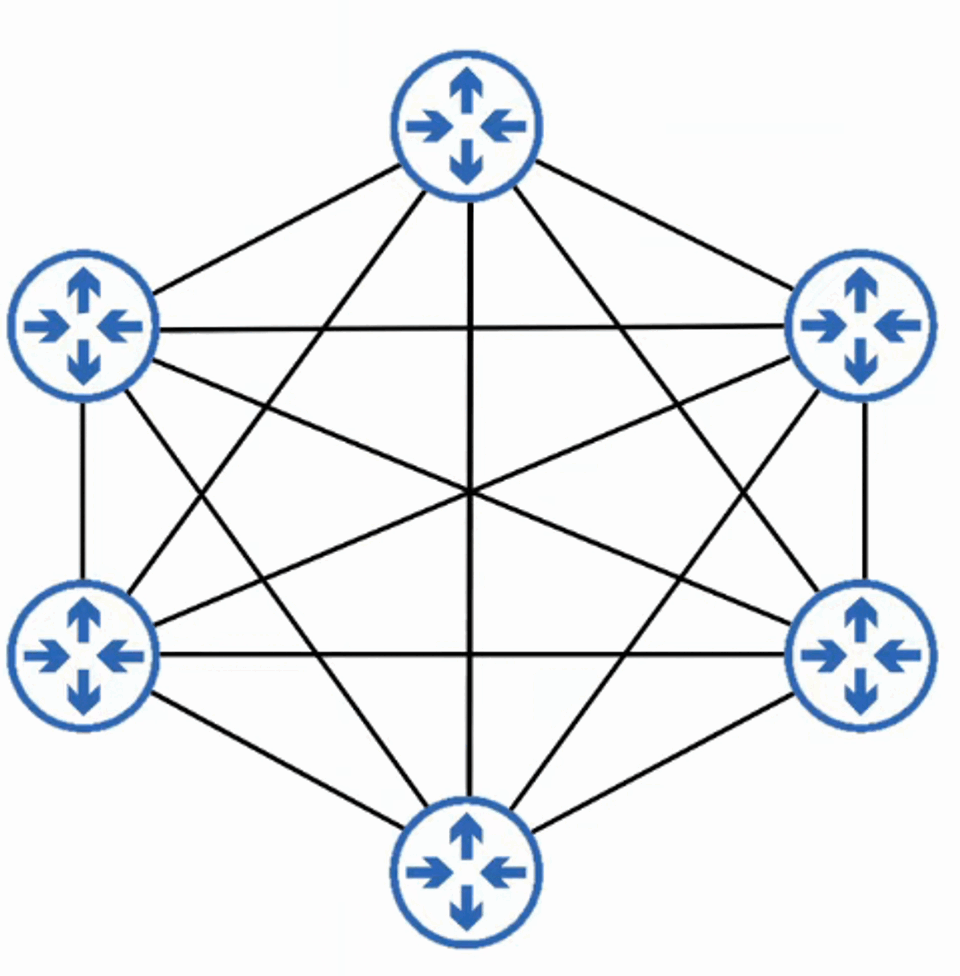
\includegraphics[keepaspectratio,alt={image}]{images/53-lan-architectures/img-002.png}}
\end{figure}

\begin{itemize}
\tightlist
\item
  PARTIAL MESH

  \begin{itemize}
  \tightlist
  \item
    When SOME DEVICES are connected to each other but not ALL
  \end{itemize}
\end{itemize}

\begin{figure}
\centering
\pandocbounded{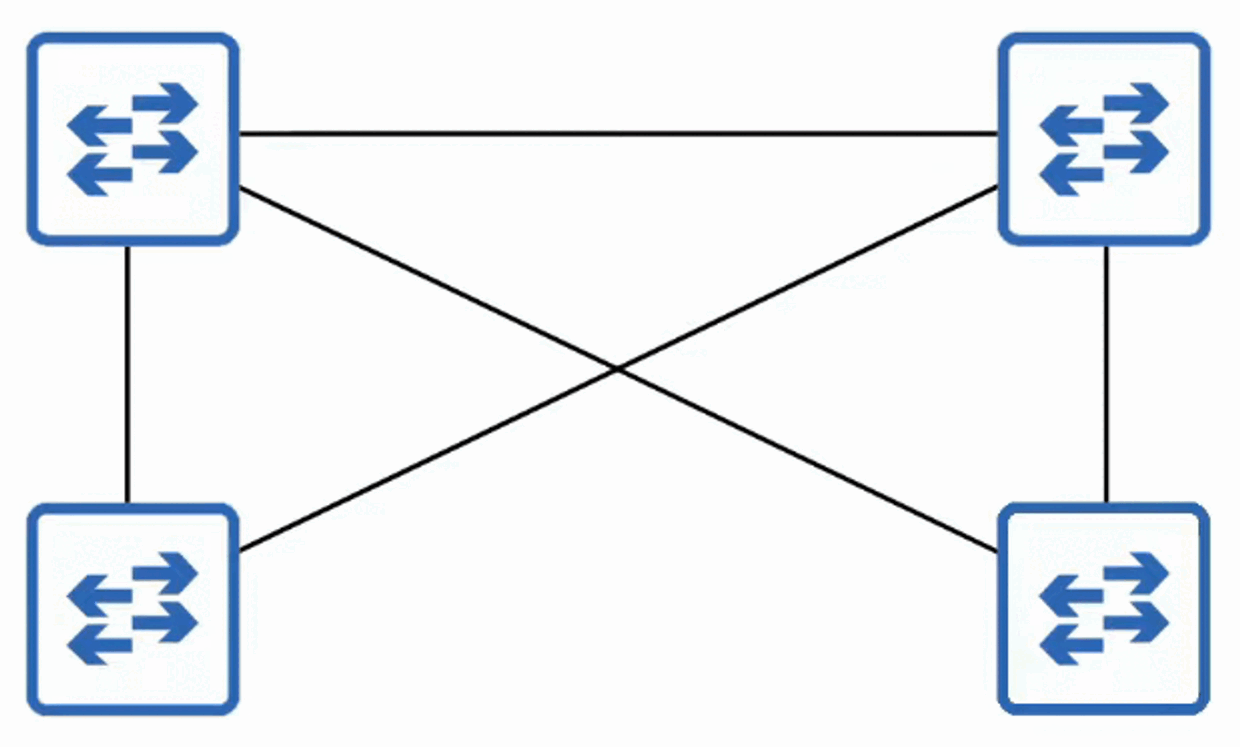
\includegraphics[keepaspectratio,alt={image}]{images/53-lan-architectures/img-003.png}}
\end{figure}

2-TIER AND 3-TIER LAN ARCHITECTURE

\begin{itemize}
\tightlist
\item
  The TWO-TIER LAN DESIGN consists of TWO Hierarchical Layers:

  \begin{itemize}
  \tightlist
  \item
    ACCESS LAYER
  \item
    DISTRIBUTION LAYER
  \end{itemize}
\item
  Also called a ``COLLAPSED CORE'' DESIGN because it omits a layer that
  is found in the THREE TIER DESIGN : THE CORE LAYER
\item
  ACCESS LAYER

  \begin{itemize}
  \tightlist
  \item
    The LAYER that END HOSTS connect to (PCs, Printers, Cameras, etc)
  \item
    Typically, ACCESS LAYER SWITCHES have lots of PORTS for END HOSTS to
    connect to
  \item
    QoS MARKING is typically done here
  \item
    Security Services like PORT SECURITY, DAI, etc are typically
    performed here
  \item
    SWITCHPORTS might be PoE-Enabled for Wireless APs, IP Phones, etc.
  \end{itemize}
\item
  DISTRIBUTION LAYER

  \begin{itemize}
  \tightlist
  \item
    Aggregates connections from the ACCESS LAYER SWITCHES
  \item
    Typically is the border between LAYER 2 and LAYER 3
  \item
    Connects to services such as Internet, WAN, etc
  \item
    Sometimes called AGGREGATION LAYER
  \end{itemize}
\end{itemize}

\begin{figure}
\centering
\pandocbounded{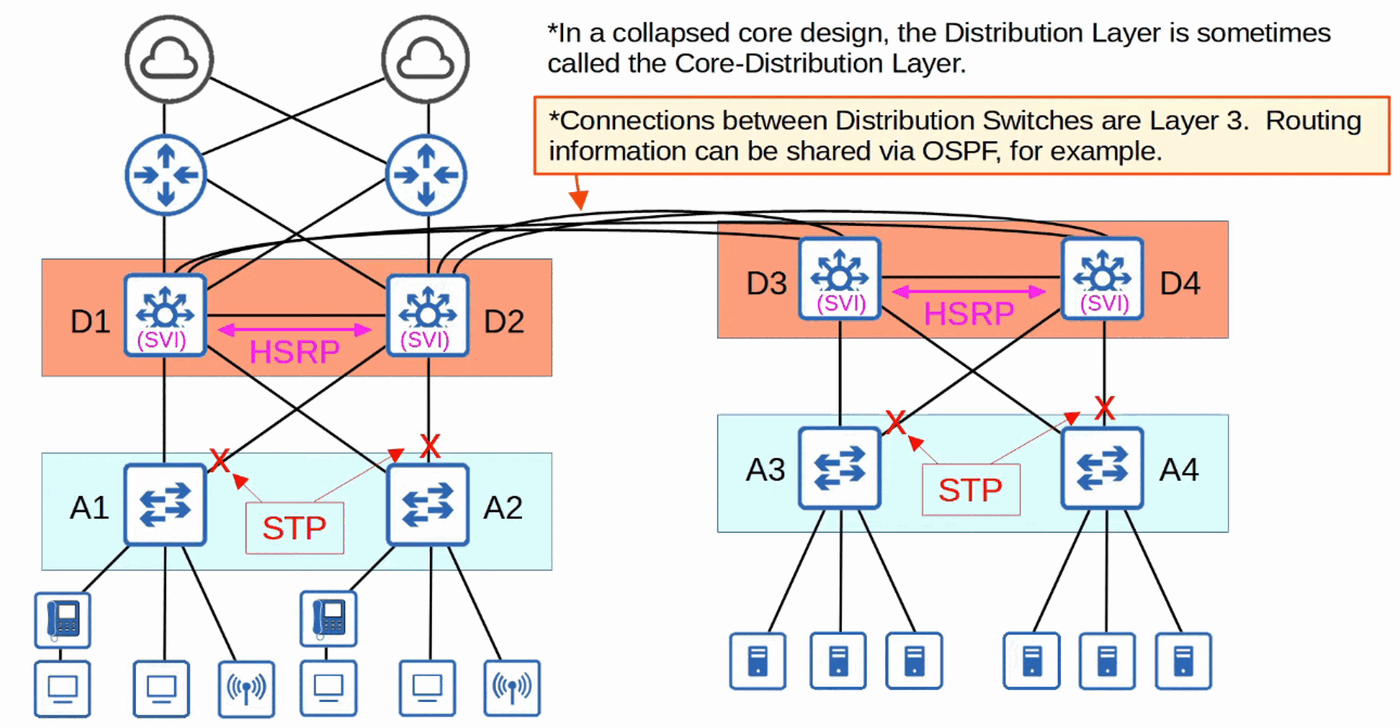
\includegraphics[keepaspectratio,alt={image}]{images/53-lan-architectures/img-004.png}}
\end{figure}

\begin{figure}
\centering
\pandocbounded{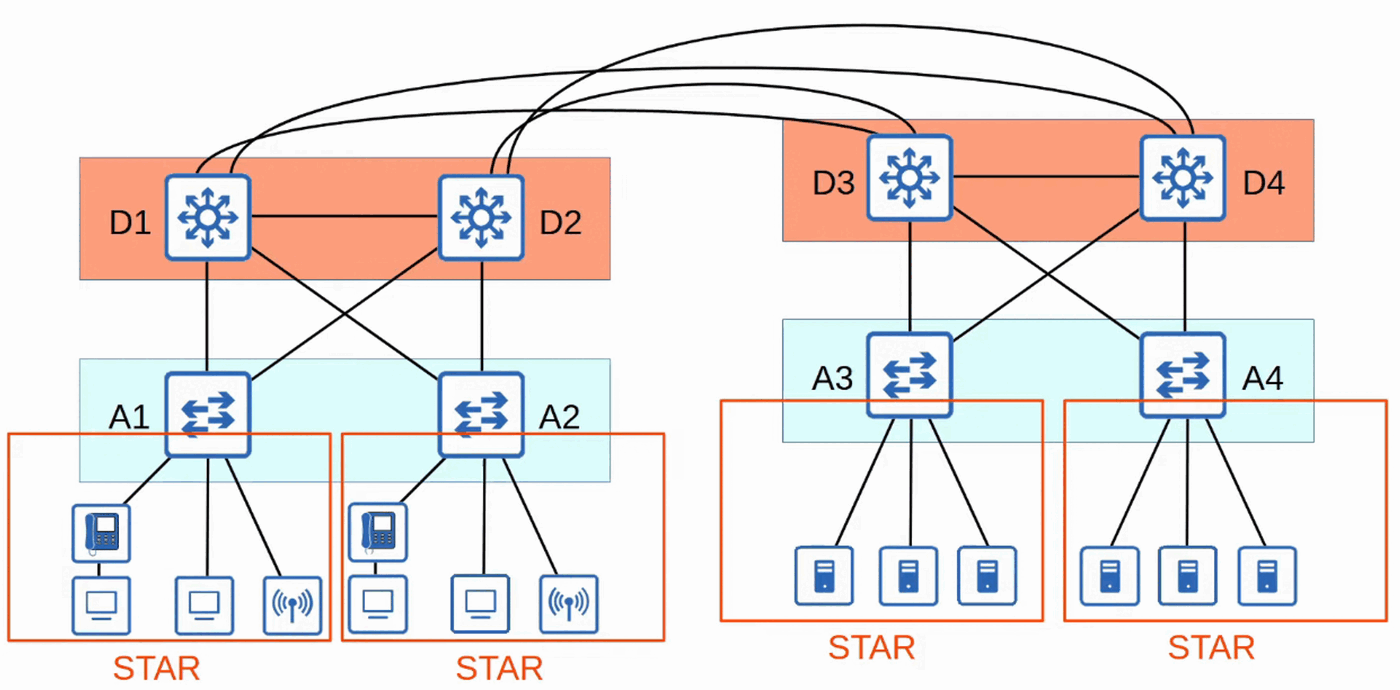
\includegraphics[keepaspectratio,alt={image}]{images/53-lan-architectures/img-005.png}}
\end{figure}

\begin{figure}
\centering
\pandocbounded{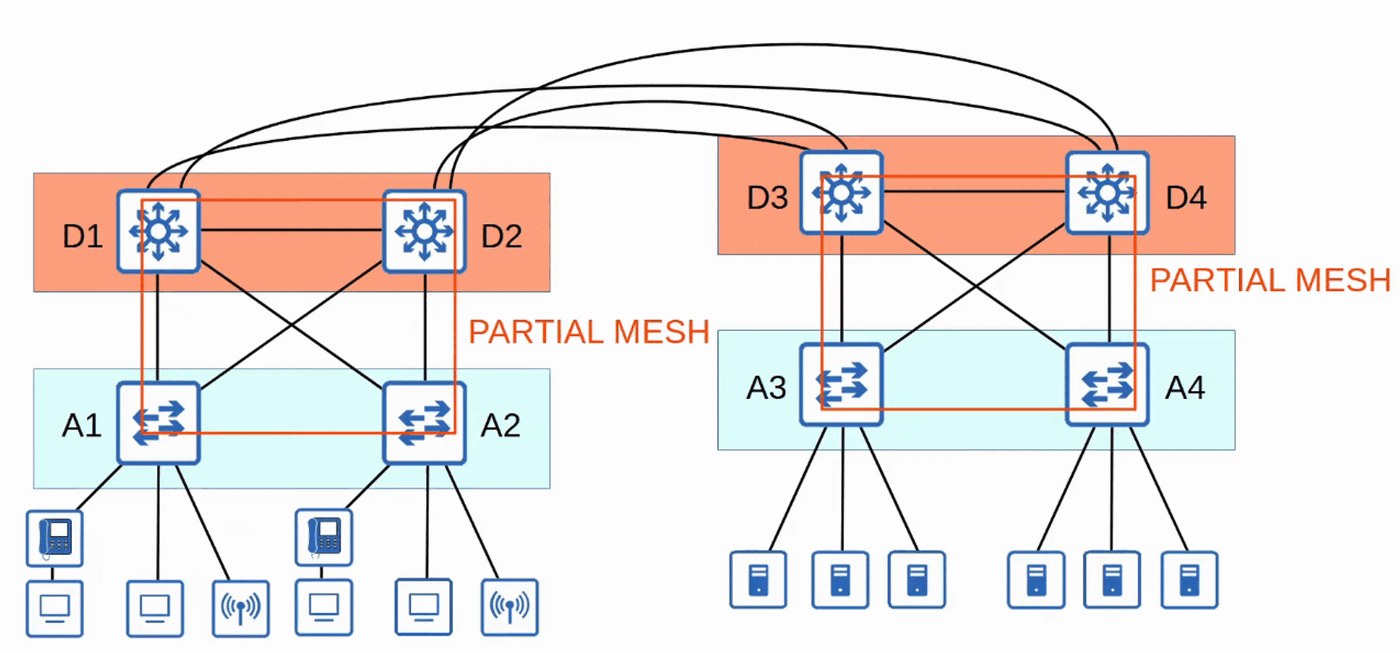
\includegraphics[keepaspectratio,alt={image}]{images/53-lan-architectures/img-006.png}}
\end{figure}

\begin{figure}
\centering
\pandocbounded{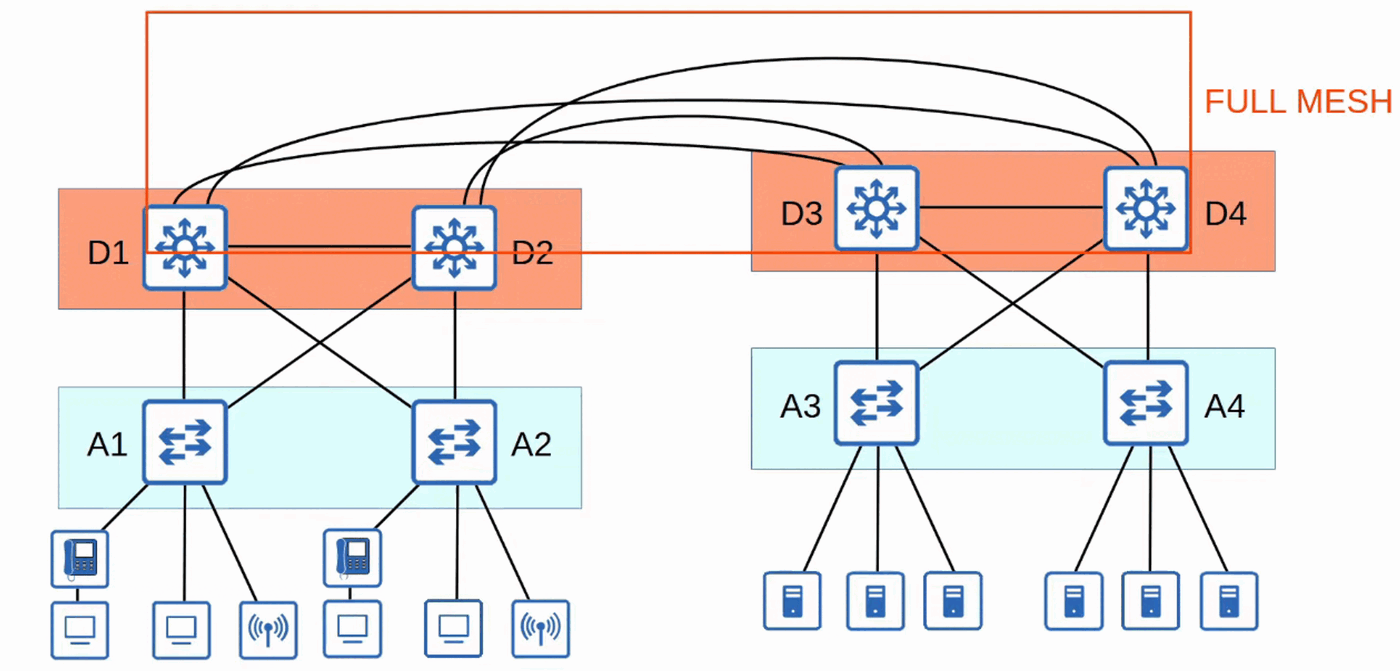
\includegraphics[keepaspectratio,alt={image}]{images/53-lan-architectures/img-007.png}}
\end{figure}

\section{Three-Tier Campus LAN
Design}\label{three-tier-campus-lan-design}

\begin{itemize}
\tightlist
\item
  In large NETWORKS with many DISTRIBUTION LAYER SWITCHES (for example
  in separate buildings), the number of connections required between
  DISTRIBUTION LAYER SWITCHES grows rapidly
\end{itemize}

\begin{figure}
\centering
\pandocbounded{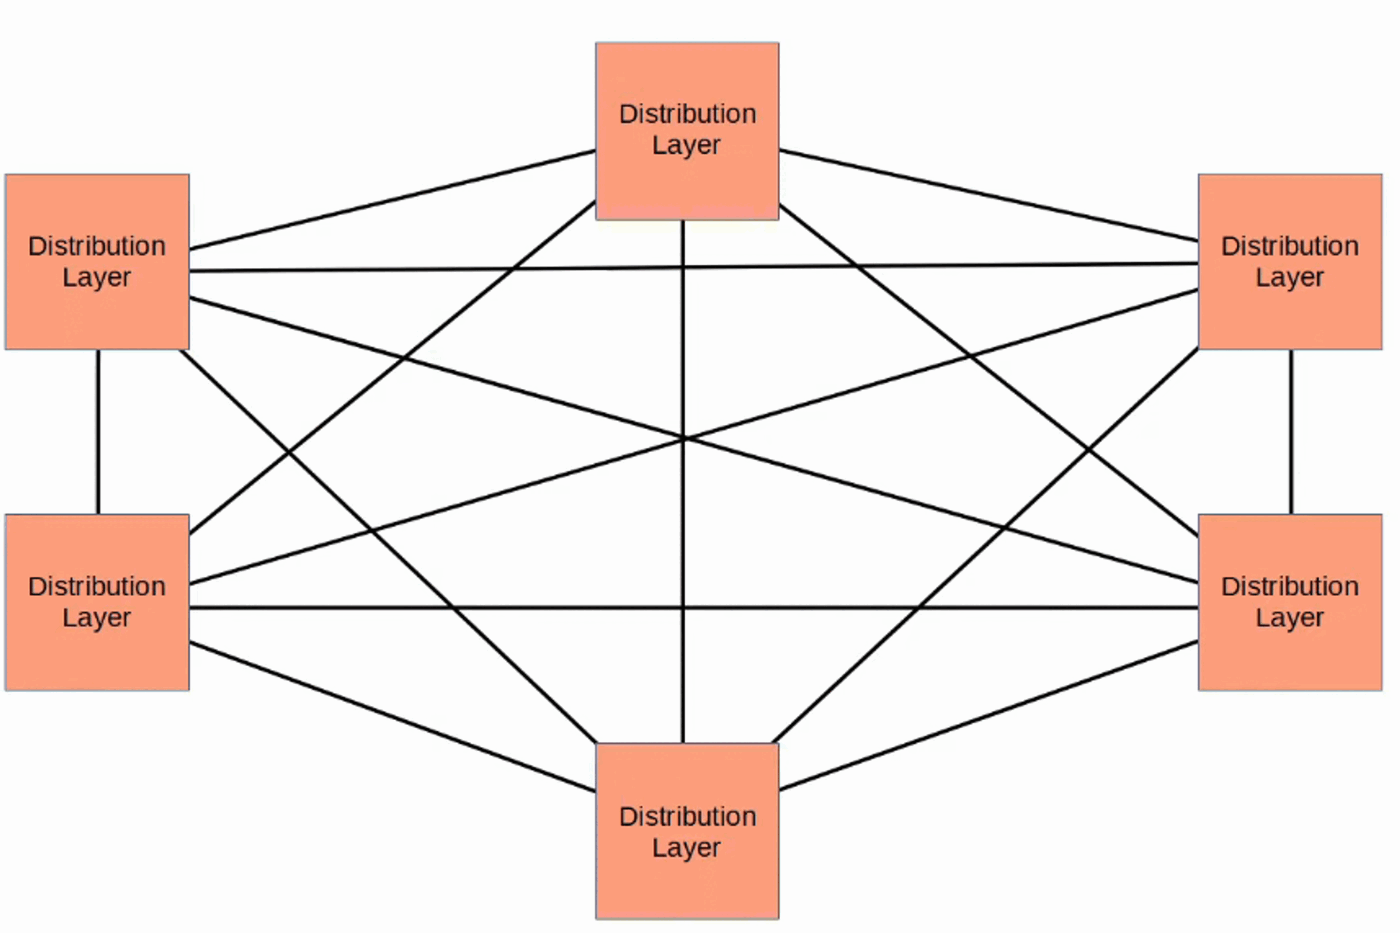
\includegraphics[keepaspectratio,alt={image}]{images/53-lan-architectures/img-008.png}}
\end{figure}

\begin{itemize}
\tightlist
\item
  To help SCALE large LAN NETWORKS, you can add a CORE LAYER.
\end{itemize}

** Cisco recommends adding a CORE LAYER if there are more than THREE
DISTRIBUTION LAYERS in a single location

\begin{figure}
\centering
\pandocbounded{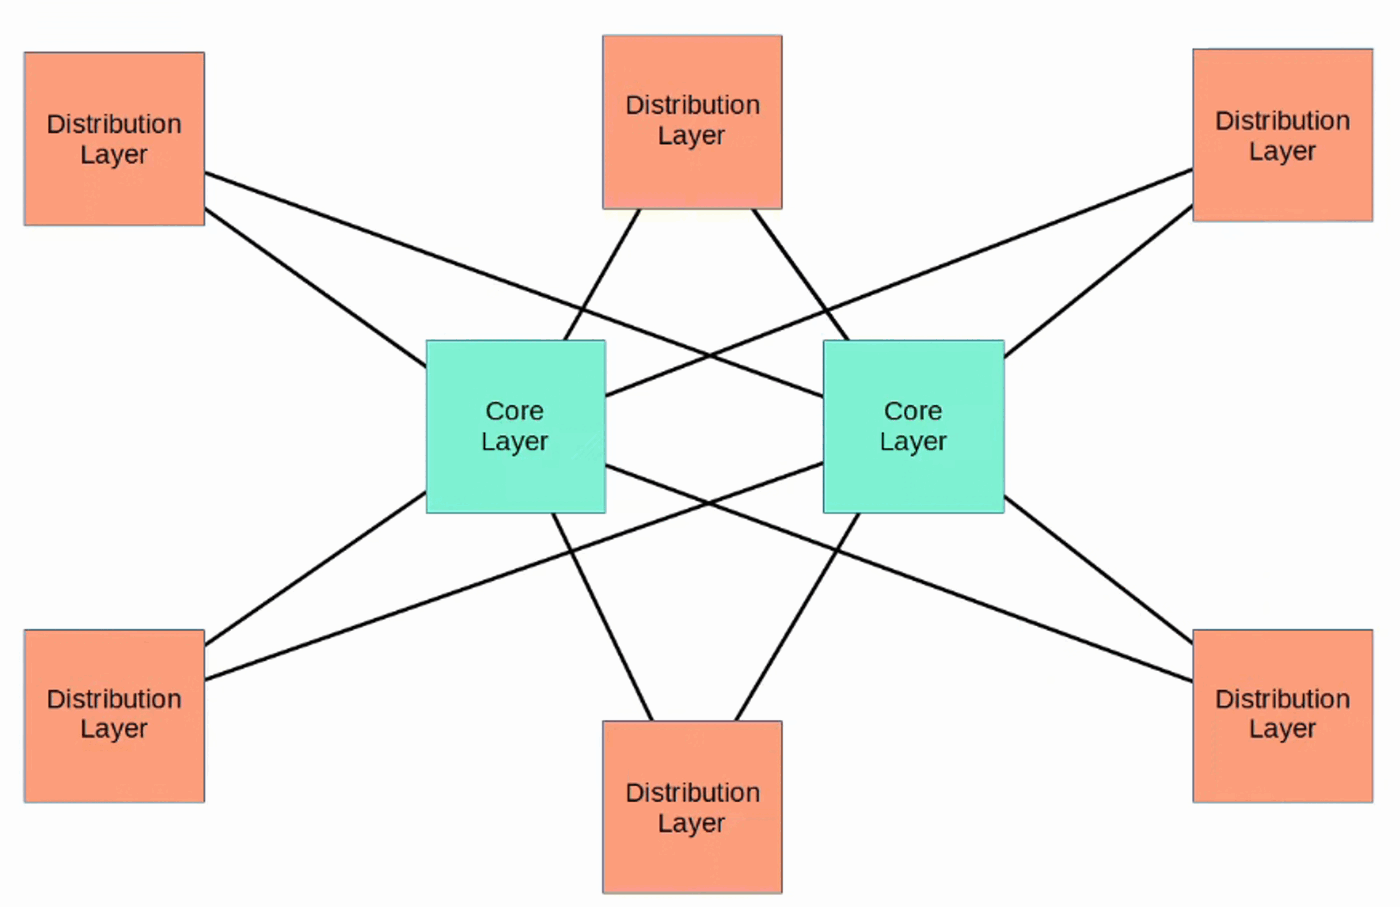
\includegraphics[keepaspectratio,alt={image}]{images/53-lan-architectures/img-009.png}}
\end{figure}

\begin{itemize}
\tightlist
\item
  The THREE-TIER LAN DESIGN consists of THREE HIERARCHICAL LAYERS:

  \begin{itemize}
  \tightlist
  \item
    ACCESS LAYER
  \item
    DISTRIBUTION LAYER
  \item
    CORE LAYER
  \end{itemize}
\item
  CORE LAYER:

  \begin{itemize}
  \tightlist
  \item
    Connects DISTRIBUTION LAYERS together in large LAN NETWORKS
  \item
    The focus is SPEED (''FAST TRANSPORT'')
  \item
    CPU-INTENSIVE OPERATIONS, such as SECURITY, QoS Markings /
    Classification, etc. should be avoided at this LAYER
  \item
    Connections are all LAYER 3. NO SPANNING-TREE!
  \item
    Should maintain connectivity throughout the LAN even if DEVICES FAIL
  \end{itemize}
\end{itemize}

\begin{figure}
\centering
\pandocbounded{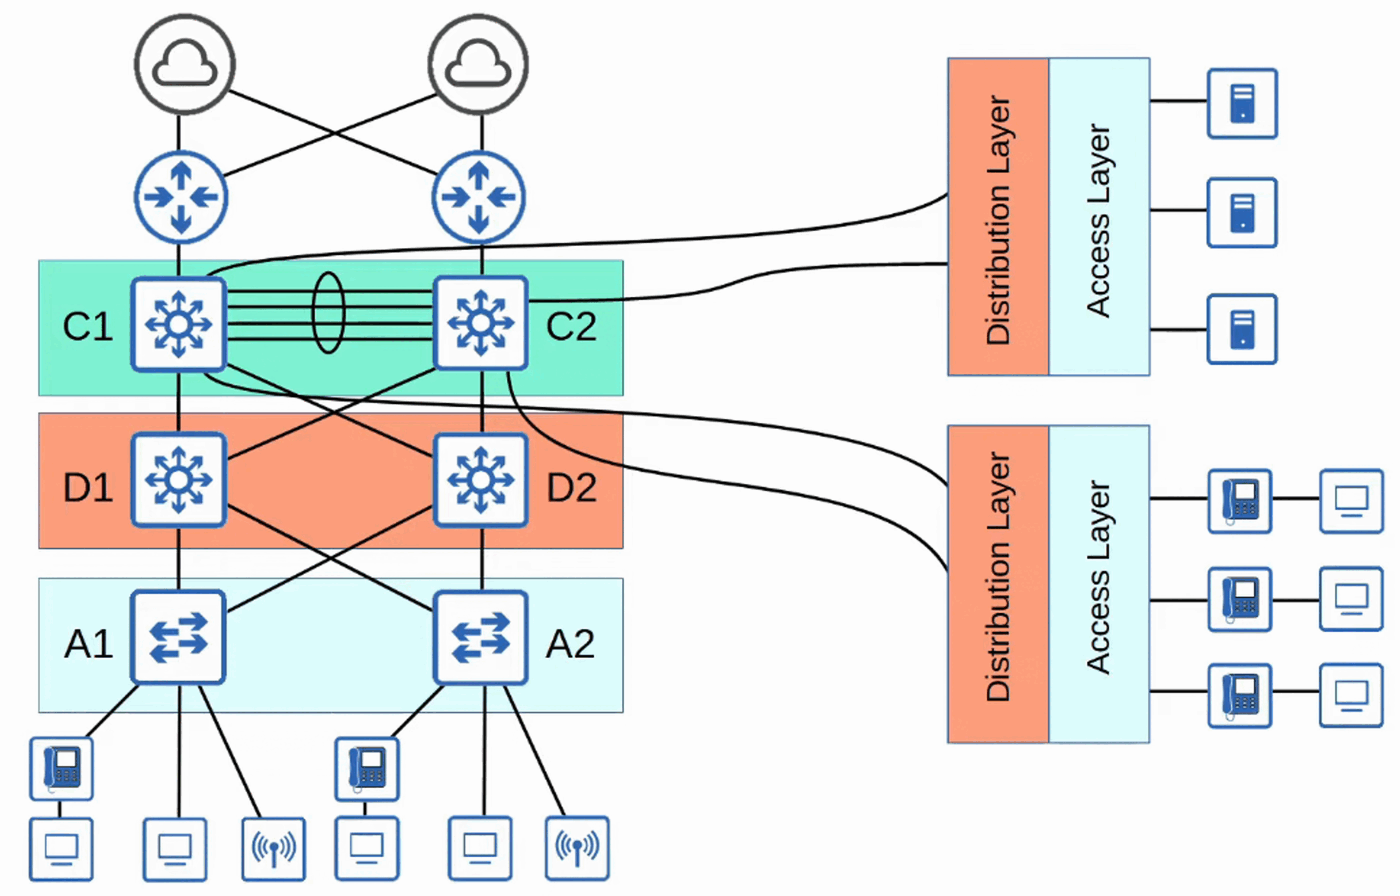
\includegraphics[keepaspectratio,alt={image}]{images/53-lan-architectures/img-010.png}}
\end{figure}

\section{Spine-Leaf Architecture (Data
Center)}\label{spine-leaf-architecture-data-center}

\begin{itemize}
\tightlist
\item
  CISCO ACI ARCHITECTURE (Application Centric Infrastructure) uses this
  architecture
\item
  DATA CENTERS are dedicated spaces / buildings used to STORE COMPUTER
  SYSTEMS such as SERVERS and NETWORK DEVICES
\item
  Traditional DATA CENTER designs used a THREE-TIER ARCHITECTURE
  (ACCESS-DISTRIBUTION-CORE) like we just covered
\item
  This worked well when most TRAFFIC in the DATA CENTER was NORTH-SOUTH
\end{itemize}

\begin{figure}
\centering
\pandocbounded{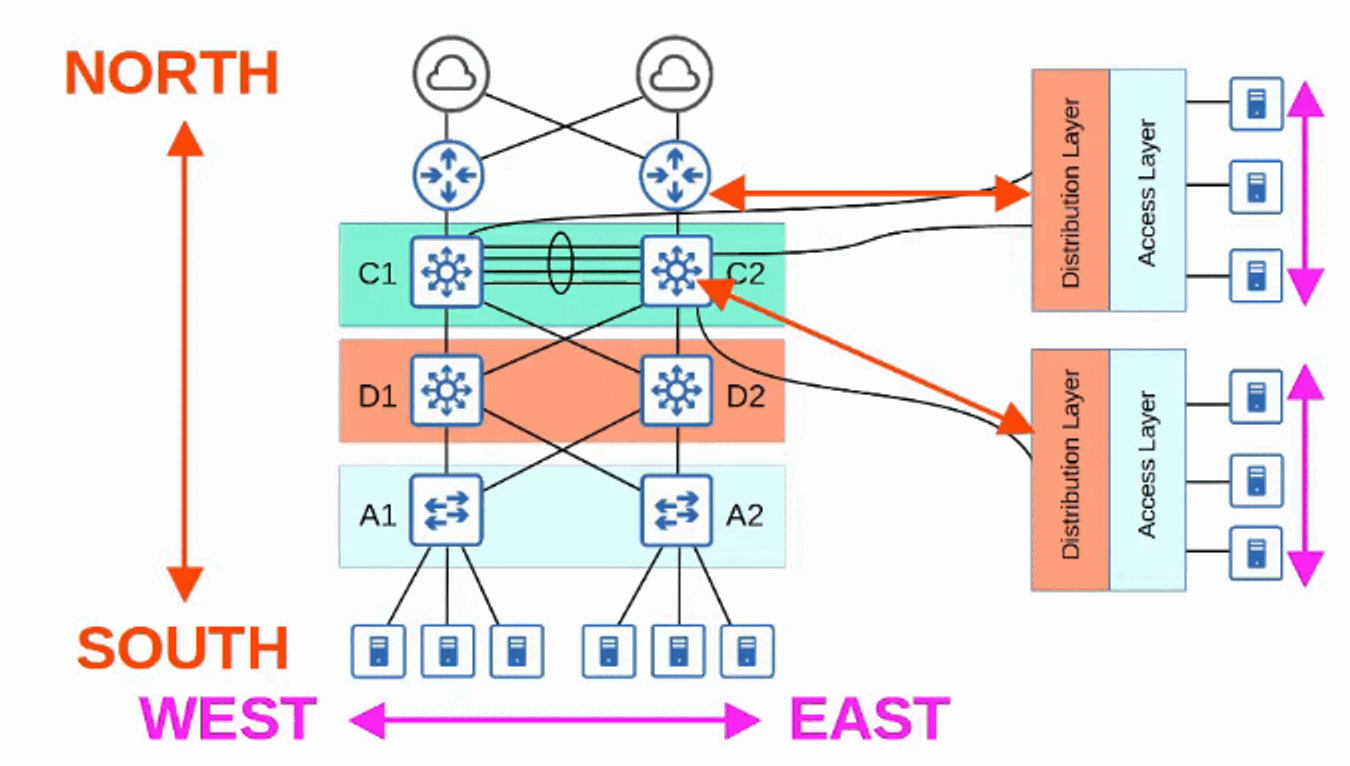
\includegraphics[keepaspectratio,alt={image}]{images/53-lan-architectures/img-011.png}}
\end{figure}

\begin{itemize}
\tightlist
\item
  With the precedence of VIRTUAL SERVERS, applications are often
  deployed in a DISTRIBUTED manner (across multiple physical SERVERS)
  which increases the amount of EAST-WEST TRAFFIC in the DATA CENTER
\item
  The traditional THREE-TIER ARCHITECTURE led to bottlenecks in the
  BANDWIDTH as well as VARIABILITY in the SERVER-TO-SERVER latency
  depending on the PATH the TRAFFIC takes
\item
  To SOLVE this, SPINE-LEAF ARCHITECTURE (also called CLOS ARCHITECTURE)
  has become prominent in DATA CENTERS
\end{itemize}

\section{Rules for Spine-Leaf
Architecture}\label{rules-for-spine-leaf-architecture}

\begin{itemize}
\tightlist
\item
  Every LEAF SWITCH is connected to every SPINE SWITCH
\item
  Every SPINE SWITCH is connected to every LEAF SWITCH
\item
  LEAF SWITCHES do NOT connect to other LEAF SWITCHES
\item
  SPINE SWITCHES do NOT connect to other SPINE SWITCHES
\item
  END HOSTS (Servers, etc) ONLY connect to LEAF SWITCHES
\end{itemize}

\begin{figure}
\centering
\pandocbounded{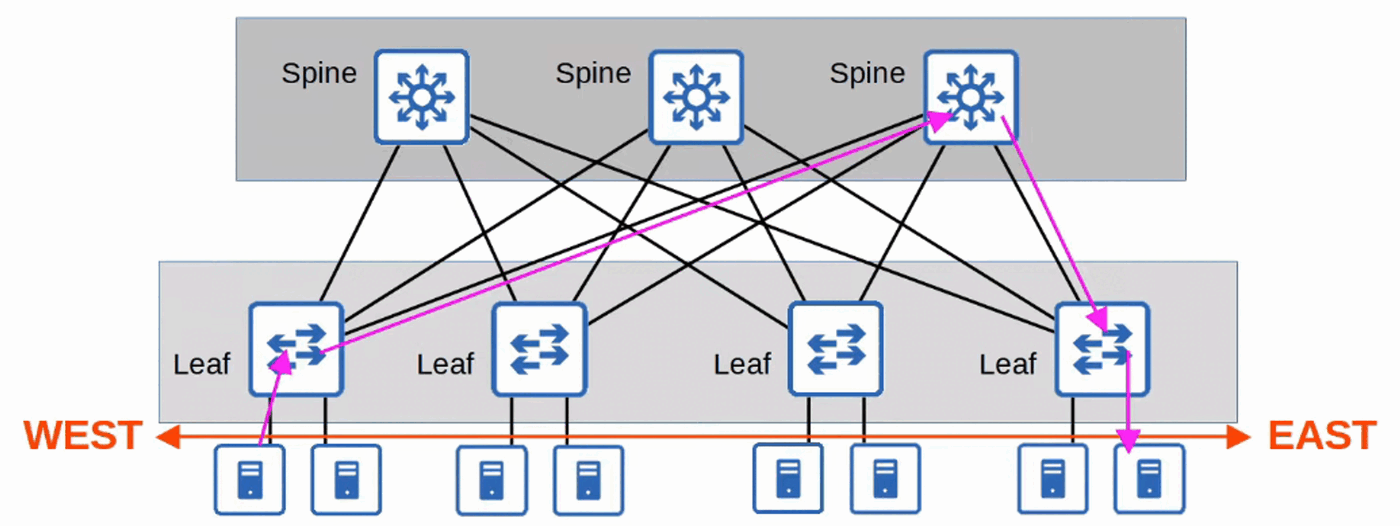
\includegraphics[keepaspectratio,alt={image}]{images/53-lan-architectures/img-012.png}}
\end{figure}

\begin{itemize}
\tightlist
\item
  The PATH taken by TRAFFIC is randomly chosen to balance the TRAFFIC
  LOAD among the SPINE SWITCHES
\item
  Each SERVER is separated by the same number of ``HOPS'' (except those
  connected to the same LEAF) providing CONSISTENT LATENCY for EAST-WEST
  TRAFFIC
\end{itemize}

\section{Soho (Small Office / Home
Office)}\label{soho-small-office-home-office}

\begin{itemize}
\tightlist
\item
  SMALL OFFICE / HOME OFFICE (SOHO) refers to the office of a small
  company, or a small home office with few DEVICES

  \begin{itemize}
  \tightlist
  \item
    Doesn't have to be an actual home ``office''; if your home has a
    NETWORK connected to the INTERNET it is considered a SOHO NETWORK
  \end{itemize}
\item
  SOHO NETWORKS don't have complex needs, so all NETWORKING functions
  are typically provided by a SINGLE DEVICE, often called a ``HOME
  ROUTER'' or ``WIRELESS ROUTER''
\item
  The one DEVICE can serve as a:

  \begin{itemize}
  \tightlist
  \item
    ROUTER
  \item
    SWITCH
  \item
    FIREWALL
  \item
    WIRELESS ACCESS POINT
  \item
    MODEM
  \end{itemize}
\end{itemize}

\begin{figure}
\centering
\pandocbounded{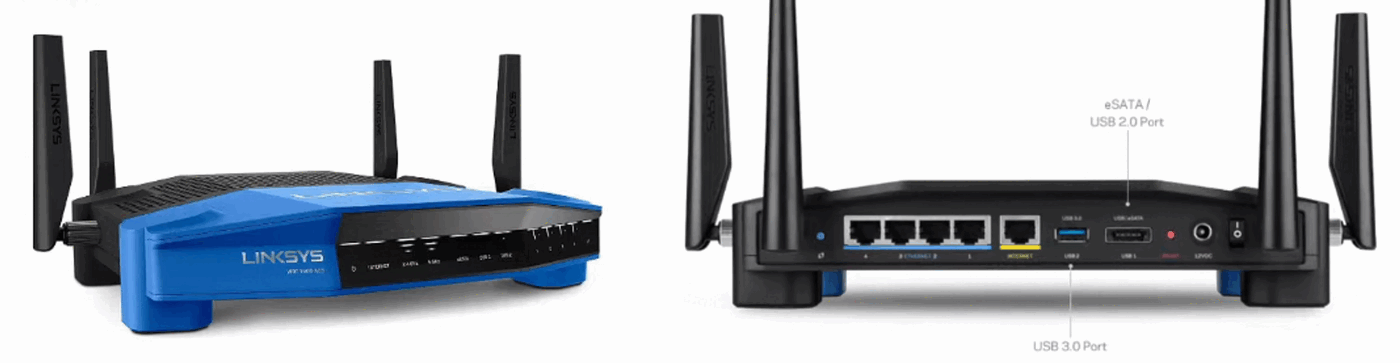
\includegraphics[keepaspectratio,alt={image}]{images/53-lan-architectures/img-013.png}}
\end{figure}

\begin{figure}
\centering
\pandocbounded{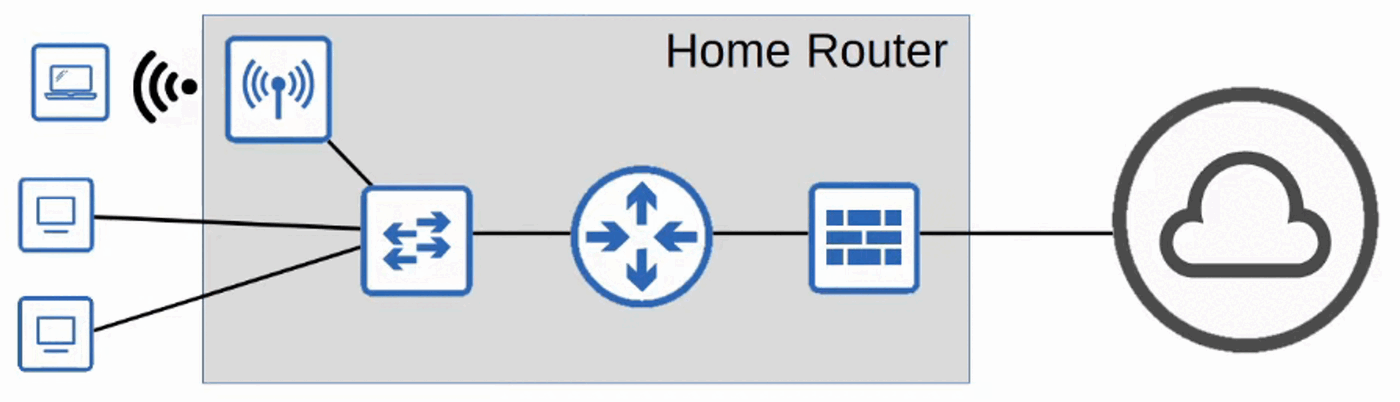
\includegraphics[keepaspectratio,alt={image}]{images/53-lan-architectures/img-014.png}}
\end{figure}
